\chapter{Imitation Games: Bypassing Google reCAPTCHA v3}\label{ch:recaptcha}

\section*{Preamble}

The history of Captchas features prominently as a cornerstone at the intersection of cybersecurity and \gls{AI}.
Introduced in the early 2000s, Captchas were conceived as a response to increasing concerns over automated abuse on the internet.
While the initial idea can be contributed to Alan Turing, it was first introduced by researchers at Carnegie Mellon University who sought to develop a system that could differentiate human users from automated bots~\cite{von2003captcha}.
The original implementations of Captchas typically involved distorted text that users would need to correctly identify, leveraging the assumption that there is a hard gap between  the visual recognition capabilities of humans over machines at the time.

The evolution of Captchas since then is marked by an ongoing arms race between developers and malicious actors.
Early successes in distinguishing human users were quickly followed by advancements in \gls{ML} and optical character recognition (OCR) technologies, which enabled automated solutions to overcome the initial Captcha designs.
This necessitated the continuous development of more sophisticated Captcha formats, such as image recognition tasks, puzzle-solving challenges, and behavioral analysis mechanisms.
Despite these advancements, attackers have persistently developed methods to break these newer Captcha systems, illustrating a dynamic progression of innovation and counter-innovation that is steadily diminishing the aforementioned gap.
This interplay and continuous mutual adaptation between attacks and defenses is found at the core of cybersecurity, \gls{AML}, and robust learning in general, accentuating their inherent affinity.
From the defensive perspective, it further highlights the persistent challenges in cybersecurity and underscores the necessity for adaptive and resilient verification mechanisms in safeguarding online environments.

This chapter has been previously published as the first comprehensive investigation of Google reCAPTCHA v3~\cite{tsingenopoulos2022captcha}.
Over a wide range of websites, web configurations, attack methodologies, and a period extending over fifteen months, we perform a black-box analysis and comprehensive evaluation of the risk scores reCAPTCHA v3 generates.
We discover that it offers insufficient protection against web automation as we are able to consistently bypass it with an evasion rate up to 99.6\%.
At the same time, we perform an analysis on how different aspects of web activity influence the score.
While static aspects like privacy settings and IP addresses have a flat effect on the score, it is also influenced by dynamic aspects directly derived from the browsing behavior of the user.
As reCAPTCHA v3 constantly monitors user interactions with the website it protects to differentiate between humans and bots, we exploit the risk score it generates to learn a general model of automated web browsing that consistently evades detection.

While the theoretical foundations of Captchas still hold, the 21st century has so far been a history of reconsidering which problems are \textit{actually} hard for AI by constantly moving the goalposts~\footnote{https://deepmind.google/discover/blog/ai-solves-imo-problems-at-silver-medal-level/}.
As text, image, and puzzle Captchas have become more difficult or involving for humans to solve than for AI, in our work we made the claim that a transition towards CAPTCHA services based on continuous behaviometric evaluation is unavoidable.
Three years after, Google reCAPTCHA has a prominent monopoly with a market share between 90-99\%.
However, as we demonstrate in this work, the ease of access to the reCAPTCHA scores inadvertently leads to a crucial vulnerability: adversaries with sufficient modeling capacity can utilize these scores to perfect the imitation of human web browsing.
The effectiveness of our approach highlights the necessity of improved bot and automation detection in zero-friction, zero-challenge Captcha.
As this type of Captcha is still and by a far margin the most widely used, the competition in differentiating between human interaction and its imitation accelerates.
We might soon reach a point were no AI-hard problem exists, something that would invalidate the premise itself of the Turing test.

So the fight against automation appears to be a losing one.
Already in 2022 almost half of all web traffic was made by bots\footnote{https://www.imperva.com/resources/reports/2023-Imperva-Bad-Bot-Report.pdf}; the advent of LLMs is only going to aggravate this phenomenon and the already deceptively large amount of generated content permeating the web today.
Moreover, it should be raising concern that the biggest ad-selling company and the biggest anti-bot company are the same: Google.
This constitutes a conflict of interest as bots are prominently used to drive engagement and click farming.
In conclusion, for the health of online communities it will be paramount to be able to prove that you are human on the web, yet if the current trend continues we are rapidly running out of tools to do so.

\section{Introduction}
The prospect of automation reshapes our notions of work, productivity, and efficiency, as it bestows us with the capacity to simplify laborious tasks or turn them obsolete.
Despite that promise, advances in automation and AI can also benefit abusive and malicious behavior in online activities, with examples ranging from social media bots \cite{chu2012detecting}, to botnets and DGA-based malware \cite{antonakakis2012throw}, and cheating in multiplayer games \cite{chow2010captcha}

In the fight against the proliferation of bots and abusive automated solutions, ``Completely Automated Public Turing test to tell Computers and Humans Apart'' or Captcha for short has proven to be as a group of approaches \cite{xu2020survey} indispensable and widely adopted as a defensive solution.
Such abusive or malicious activity is often motivated by direct financial incentives so automated solutions for Captcha -- or poorly compensated human solvers -- have always been on high demand.
In response, Captcha developers have consistently tried to stay one step ahead in the competition between human problem-solving skills and their algorithmic approximation.
This competition has elicited various fundamental and ad-hoc changes in Captcha designs that can render a solver ineffective, as each solver is usually crafted for specific types of Captcha.
The arms race is in constant flux, with adversaries devising novel solvers and Captcha services gravitating from text-based to image-based challenges.
Recently, the interactive part of the Turing test, that is the challenge itself, is gradually being removed as it becomes progressively more challenging and time-consuming for humans to solve.
After all, a Captcha challenge maintains its practical utility insofar as it is easy for humans but difficult for automated approaches to solve.

Nevertheless, the burgeoning capabilities of AI, particularly in computer vision and image segmentation, call the security offered by text and image based Captcha into question.
Regarding text-based Captcha, previous work has demonstrated that a generic solution can be used to solve new Captcha schemes without requiring an ad-hoc approach~\cite{bursztein2014end}.
At the same time, automated solving has been shown possible on the full range of challenges presented by Google's reCAPTCHA v2, challenges that are primarily image based \cite{sivakorn2016robot}.
As automated solutions proliferate, the foundations upon which challenge-based Captcha builds are unstable.

A recent version of Google reCAPTCHA is v3 and the first to offer completely frictionless user verification by simply observing the user and the information they generate.
The motivation behind v3 is twofold, to minimize the interruption in user experience and at the same time conceal the exact nature and presence of the challenge: it is the next move in the imitation game.
In place of an explicit challenge that calls for a solution, reCAPTCHA v3 service returns a score to the back-end based on interactions within the website, and enables the host to take appropriate actions based on that score.
In the absence of an explicit challenge, the whole web session of the user becomes the challenge.
In fact, v3 constitutes a paradigm shift over all previous approaches in Captcha systems so far: it verifies users without interrupting or presenting to them a challenge.

We set out to explore three key research questions:
Can we disentangle the data that reCAPTCHA v3 is observing in order to determine how they influence the final score?
Can we evade reCAPTCHA v3 detection by simulating human behavior and if yes, under which conditions is the above possible?
Finally, can we utilize reCAPTCHA v3 as an oracle in order to learn a general evasive model of online browsing behavior?
An affirmative answer to these questions would indicate significant vulnerabilities in reCAPTCHA v3.

To that end, we build an automation framework that is able to navigate the web in a GUI-enabled manner.
As a first step, we host our own website protected by reCAPTCHA v3 as a testbed and in order to evaluate the extent that it can be exploited.
Then we step into the wild; we scale up our experiments to two public websites that are not under our control with considerable daily traffic.
To enable our subsequent automated experimentation, we first perform a manual analysis of how reCAPTCHA v3 functions as a black-box.
Specifically, we observe how various aspects of the web browsing behavior affect it, from less fluctuating properties like cookies and privacy settings to more dynamic ones like mouse control and timings.
Finally, we build a substitute model that shadows the reCAPTCHA v3 risk analysis system.
Then we perform an explainability analysis on it in order to evaluate how different browsing aspects contribute to the score and thus how adversaries can potentially exploit it.

Over an extensive period of both manual and fully automated experiments, we show that it is possible to consistently avoid detection in widely varied web environments.
Additionally, we show that it is possible for an adversary to exploit the implicit challenge itself in order to learn a web browsing behavior with up to a 99.6\% evasion rate against detection.
To actualize that, we leverage a \gls{RL} methodology as the agentic component of our automation framework, which is trained by interacting in an online manner with the websites in question, requesting verification, and using the received risk score as the reward signal.
The task and the environment are formulated in a manner that allows a general evasive model to be learned, something that can subsequently enable various automation attacks, from fraudulent transactions to credential stuffing and click fraud.

As the gap between humans and AI agents diminishes, Turing tests are shifting towards continuous observation and verification, and any such test that can be consistently queried will in practice enable the further diminishing of this gap; bots are inadvertently created in our own image.
With reliable and pervasive human verification on the web remaining essential, we propose potential mitigations, however without another paradigm shift these can be only a temporary deterrence.

The contributions of our work can be summarized as follows:
\begin{itemize}
\item At the time of publication, this is the first comprehensive study of reCAPTCHA v3 along with its advanced risk analysis system.
\item We propose a novel RL-based automation framework that consists of three different types of agents, each more capable than the previous in learning human web browsing behavior.
\item We collect and study verification scores over a period of fifteen months in various web environments, and perform a state-of-the-art explainability approach to quantitatively evaluate how different factors influence the score.
\item We perform an extensive evaluation of our proposed approach, on three different websites.
The most comprehensive agent -- one that incorporates navigation, typing and scrolling as capabilities -- successfully transfers to third-party websites reaching an evasion rate up to 99.6\%.
\end{itemize}

The remainder of the chapter is structured as follows:
Section \ref{sec:related} provides the necessary background on the domain and reviews the related work.
Section \ref{sec:recap} analyzes how reCAPTCHA v3 operates, from its source code to its web mechanisms.
Section \ref{sec:approachre} describes the web environments and our automation framework.
In Section \ref{sec:evaluationrere} we elaborate on our experimentation and analyze our results.
In Section \ref{sec:discussionre} we discuss insights, limitations and challenges, before concluding in Section \ref{sec:conclusion}.

\section{Related Work}
\label{sec:related}

Completely Automated Public Turing test to tell Computers and Humans Apart, or CAPTCHAs as they are more commonly known were initially conceived as challenge–response tests to determine whether an agent interacting with a website is human or machine.
While it is unclear who came up first with the concept, which has been around since the late nineties~\cite{naor1996verification}, the term Captcha itself initially appears in the work of von Ahn et al. in 2003~\cite{von2003captcha}.
What is of particular interest in this work is that it constitutes the first exploration of utilizing AI problems as security primitives, drawing parallels with prime factorization in cryptography.

The first generation of Captcha schemes was based around recognizing combinations of distorted characters.
The straightforward assumption is that it would be easy for humans to recognize the characters and complete the challenge, but difficult for AI.
Text-based Captcha also proved instrumental in digitizing old archives and books, as many of the challenges presented to the users were texts flagged by optical character recognition (\gls{OCR}) as unreadable.
In terms of individual characters, previous work has been demonstrated that \gls{ML} algorithms consistently outperform humans in recognizing them~\cite{chellapilla2005computers}.
The resilience of a text-based Captcha to automated solving therefore lies in the difficulty of segmentation: creating segments that contain individual characters~\cite{bursztein2014end}.
As anticipated, this has led to an arms race between Captcha creators and automated solving attacks, by applying new distortions and creating new segmentation techniques tailored to these distortions respectively~\cite{cruz2012breaking}.

Around 2014, Google introduced a new reCAPTCHA mechanism purported to be more human-friendly and secure.
This version of reCAPTCHA which is still active to this day is known as v2, while in 2018 Google retired reCAPTCHA v1 that was based on text character recognition; it was no longer fit for purpose as it was demonstrably more difficult to solve for humans than AI.
Unlike its predecessor, the reCAPTCHA v2 challenge consists of two sequential parts: a system that performs the initial risk analysis, and in case this analysis flags traffic as suspicious, then the user will be prompted to solve a Captcha challenge.
The challenges presented in the latter case are image recognition problems, e.g. the user is asked to select among a collection of pictures the ones that contain the designated object or property.

AI problems were not always used as fundamental primitives in computer security.
In their seminal work, von Ahn et al. \cite{von2003captcha} assert that the advantages of using hard AI problems as a means for security are twofold.
If the problem cannot be solved, then it remains as a reliable method for distinguishing humans from AI.
If the problem can be solved, then that is by itself beneficial in the progress towards stronger AI.
In the case of image- and text-based Captcha, contemporary AI solutions are capable of better than human segmentation and recognition in both images and texts~\cite{bursztein2014end, sivakorn2016robot, karpathy2015deep}.
As the demand for reliable human verification online is high and will not subside in the foreseeable future, we inquire as to how can the Turing tests stay one step ahead.

One such approach is Captcha based on game playing, also known as Dynamic Cognitive Games (DCG), that attempts to make Captcha solving a fun activity for the user~\cite{mohamed2014three}.
Such solutions are still vulnerable to automated solving and additionally require a higher engagement from the user which can be frustrating while browsing.
While hard AI problems are becoming easier to solve, a paradigm shift takes place in contemporary Captcha solutions. 
When bot detection~\cite{d2014avatar} and biometric authentication~\cite{fridman2015multi} transition from one-shot to continuous, the competition between detection and evasion accelerates.
As bot detection systems start relying on behaviometrics and constant checks to detect bots, the extension of the challenge over the temporal domain introduces a new vulnerability.
When designing new Captcha, the paradigm is no longer an incremental contest between challenge design and ad-hoc, tailored solutions, but between two AI-enabled systems that engage in a constant, interactive competition, where one's decisions become the other's information.

\subsection{Evasion}

Currently, there are several approaches available for unsuccessfully advancing past Captchas challenges: employing some \gls{ML} methodology to solve the challenge or exploit bugs in the implementation to bypass the challenge completely.
A third option is through websites like anti-captcha or 2captcha that employ cheap human labor~\cite{weng2019towards}; such availability has led to the emergence of Captcha solving markets~\cite{motoyama2010re}.

Bug exploitation is typically short-lived as bugs and workarounds are quickly patched.
The most substantial threat is posed by automated solutions to the challenge.
Bursztein et al.~\cite{bursztein2014end} introduced a generic text Captcha-solving algorithm based on \gls{RL}, demonstrating in that way that text based CAPTCHAs schemes are inherently vulnerable.
Their approach obviates any hand-crafted components, so it generalizes to new text-based CAPTCHA schemes, and assigns a score to all possible ways of segmenting the text.
Being one of the first approaches to use \gls{RL} in Captcha solving, they ask humans to annotate segments that have been misclassified and the \gls{RL} algorithm learns from feedback and selects the segmentation that gives the highest score.
This conclusion was strengthened by Ye et al.~\cite{ye2018yet} which presented a deep learning-based approach that could solve with high success rate 11 different text Captcha schemes commonly used at the time by the top-50 popular websites.

Regarding image Captcha, Sivakorn et al.~\cite{sivakorn2016robot} conduct a comprehensive study of reCAPTCHA v2 by exploring how the risk analysis process is influenced by various aspects of the request: browsing history, Google account, geolocation and browser checks.
They also design a module that upon receiving a challenge automatically extracts the images that are subsequently passed to popular annotation tools like Google Reverse Image Search and Clarifai.
They also conclude that \gls{ML} capabilities have advanced to a point where distinguishing between humans and bots through such challenges is infeasible.
While reCAPTCHA v2 is constantly adapted to account for new attacks, by being based on image recognition challenges it still remains fundamentally vulnerable.
The latest work on attacking v2 is from Hossen et al.~\cite{hossen2020object}, where they propose an automated, object detection based attack, and successfully solve most (83.25\%) of the image-based reCAPTCHA v2 challenges.

Furthermore, even audio challenges did not prove resilient to automated solutions, as the authors in~\cite{bock2017uncaptcha} have developed an AI-based solution to solve audio reCAPTCHAs.
Finally, a recent work~\cite{dionysiou2020sok} systematizes the knowledge around the broad domain of automated Captcha solving that includes text, image, audio and video challenges.

\subsection{Behaviometrics}

Up to this point, Captcha challenges have proven inadequate to effectively differentiate between humans and bots as they can be consistently bypassed by automated solutions.
This has led researchers to consider introducing behavioral biometrics, or behaviometrics for short, into the Captcha challenge.
The idea to utilize behaviometrics to differentiate between legitimate users and bots has existed for some time~\cite{yampolskiy2006use, chu2013blog}.
Collecting behavioral data is considered advantageous by merit of being unobtrusive while offering accurate identity verification.
The first work to have successfully incorporated mouse behaviometrics as part of a Captcha challenge was by D'Souza et al.~\cite{d2014avatar}.
Specifically, they extract mouse features such as movement speed, click time, and angle of curvature, in order to build what they describe as Mouse Dynamic Signature (MDS) profiles.
A \gls{SVM} classifier is subsequently trained on such profiles that achieves near-perfect accuracy in bot detection.
Behaviometrics offer several advantages over typical Captcha challenges as they do not interrupt user experience and conceal the nature of the challenge, a deterrence against automated solutions.

Another advantage of zero challenge Captcha is that, since it does not interrupt the user, it can be continuously evaluated and thus over time and during a web session it can lead to more accurate detection.
This property draws a direct parallel between such Captcha and active authentication, which is the process of continuously verifying a user based on their ongoing interactions with a computer.
In~\cite{fridman2015multi}, Fridman et al. present a methodology where they can continuously and successfully authenticate users based on multiple modalities: mouse and keystroke dynamics, as well as stylometry.
The application might be different in that case, that is intruder detection, but the principle is directly applicable to the context of bot detection; telling a human apart from another is not that different from telling a human apart from a simulacrum.
In the most recent work on behaviometric Captcha, Acien et al.~\cite{acien2020becaptcha} build a scheme that works solely on mouse trajectories, and they show that a mouse-based CAPTCHA can be a highly dependable bot detection system.
According to its documentation, Google reCAPTCHA v3 hints on the use of behavioral data, however before attempting to bypass it we require an in-depth investigation of the data it collects and its underlying mechanisms.

\section{reCAPTCHA v3}
\label{sec:recap}

Version 3 is one of the latest additions in the range of Google's reCAPTCHA services, the first of the CAPTCHAs to achieve that without any user friction.
It employs an advanced risk analysis system to generate a score ranging from 0 that is very likely a bot to 1 that is very likely a human, based on information collected and overall interactions within a website.
The back-end can request verification at any point or time a user takes a specific action within the website.
At first glance, the transition from a conspicuous, distinct Captcha challenge to an obfuscation of where or what exactly is the challenge can be considered advantageous for both users and administrators, for a number of reasons: it does not interrupt user experience, it obfuscates the exact nature of the challenge, and in place of a binary decision it returns a more granular score that is delegated to the back end.

There is potentially another reason for the transition from one-shot, explicit challenges, to a model more akin to continuous authentication by observing interactions and generating intermittent risk scores.
While \gls{AI} might be constantly closing the ``hard for AI - easy for humans problem'' gap, von Ahn et al.~\cite{von2003captcha} point out that no matter how small this gap becomes, as long as there remains one between the human and the AI ability with respect to some problem, this problem can be used as a primitive for security.
Rather than asking the user to solve a problem once, we can ask them to solve the problem multiple times.
Even better, if the problem does not require any explicit input from the user and does not interrupt them, it can be solved continuously.

As is the case with v2, the latest version of reCAPTCHA embeds a widget in the website that it protects while it offers granular and adaptive scoring to the web admins and frictionless and uninterrupted experience to the user.
Naturally, to prevent analysis from third parties, the widget's JavaScript code is obfuscated.
The JavaScript code from reCAPTCHA v2 has been de-obfuscated and has provided insights as to what information exactly is being recorded and forwarded to Google\footnote{https://github.com/neuroradiology/InsidereCAPTCHA}.

\subsection{Source Code Analysis}
In this section we describe the details on deobfuscating the source code of reCAPTCHA v3, identifying the observed information, and verifying if that information can be programmatically intercepted and manipulated.
The JavaScript code that implements reCAPTCHA v3, and that always kicks-off at page load, is polymorphic and protected by virtualization-based obfuscation.
We managed to hook the debugger and witness the various events being logged and processed, yet we were unable to reverse their encoding or meaningfully control the final response.
Our attempts were hampered further by multiple levels of timeouts and sanity checks, and while it was possible to directly manipulate some relevant variables, we did not manage to affect the score, most likely due to the variables being manipulated either at the wrong time or in the wrong way. 

More specifically, we utilized the well-known BurpSuite\footnote{https://portswigger.net/burp} to capture the request responsible for sending the reCAPTCHA v3 JavaScript code back to the browser and, each time, insert a breakpoint in the code.
The exact position of the breakpoint was determined via trial-and-error, as pausing in certain locations caused the multi-threaded code to become desynchronized.
Subsequently we coarsely iterate through the code and see clear signs of session-related variables, such as the respective Navigator object, being manipulated.
However, manually modifying the values of said variables did not have an observable effect on the score. 
By inspecting the named variables in the source code we identify a multitude of strings that relate to user browsing behavior; ``mousedown'', ``mouseup'', ``mousemove'', ``mouseover'', ``mouseenter'', ``keydown'', ``keyup'' and others.
This information can pertain to functionalities separate from how the score is generated, or even function as a red herring.

While manipulating this information at a low-level by capturing requests and perturbing session variables proved ineffective, our low-level analysis yielded insights on how to affect the score through a higher level abstraction.
The further specification of our automated solution was facilitated through contrasting what is implicitly or explicitly monitored by the source code on the one hand, and the wealth of information every user generates continuously and in principle unconsciously during a web session on the other.
IP address, the presence of cookies, the user-agent string, all embody the invariable part of the session information collected.
The variable part is user dynamic behavior -- timings, mouse and keyboard dynamics -- which has the potential to affect the score; the goal of our approach is to simulate a general web browsing behavior that also successfully evades detection.
As security through obscurity is a fundamentally flawed approach, through our implementation that can control all the above information, we put our hypotheses to the test.

\subsection{Website Integration \& Evasion}
Unlike reCAPTCHA v2 where the user is required to click the ``I am not a robot'' checkbox, v3 offers two ways of generating the token that is subsequently verified by Google.
It can be generated either by binding the challenge to a button within the website, or by programmatically invoking it when the user takes a specific action while browsing the website.
The latter offers higher granularity on where exactly does abusive behavior actually occur, and a detailed summary for these locations in Google's admin console.
In order to adapt the risk analysis for each website, Google's admin console requests to specify an action name in each place that reCAPTCHA verification is executed, implying that separate statistics are kept for each such action.
After the token is generated, the back-end forwards it to Google together with the website's sitekey in order to be verified.
Finally, a score $s \in \{0.1,0.3,0.7,0.9\}$ is returned to the back end, where the decision on how to act on it is transferred to the administrator.
Based on the score, the context, and the adjustable threshold, various actions can be taken, from requesting further verification or downright blocking the traffic.
This verification flow is shown in Figure \ref{flow}.

\begin{figure}[htbp]
\centerline{\includegraphics[width=0.8\columnwidth]{reCAPTCHA.png}}
\caption{reCAPTCHA v3 verification workflow.}
\label{flow}
\end{figure}

Currently, Google ReCAPTCHA solutions are deployed in 37.8\% of the top 10K and about 13.2M total websites\footnote{https://trends.builtwith.com/widgets/reCAPTCHA-v3}, while the have about 90\% of the Captcha market share\footnote{https://trends.builtwith.com/widgets/captcha}.
Specifically for v3, it was launched in October 2018 and at until the time this research was carried out (2021), there had been a puzzling lack of research on it.
% it was deployed on 8.5\% of the top 10K and about 1.1M in total, 
One exception was by Akrout et al.~\cite{akrout2019hacking}, where they propose a methodology to bypass reCAPTCHA v3.
However, there were several limitations that we addressed with this work.
The authors did not mention how they handle the lack of the ``I am not a robot'' checkbox -- or of any other challenge for that matter -- in reCAPTCHA v3; after all the goal in v3 is to offer completely frictionless, uninterrupted web experience.
In the absence of such a transparent challenge and response interface that can be consistently queried, a methodology that endeavors to learn on it requires first the definition and then the implementation of such an interface.
Secondly, pixel by pixel mouse control and mouse trajectories as a composition of multiple smaller ones are insufficient to describe realistic, human-like mouse dynamics.
Finally, mouse dynamics are just one aspect of human browsing behavior; we explore a more general approach that includes timings, scrolling, and keyboard strokes, as well as the effect these have on the score. 

The research question behind~\cite{akrout2019hacking} is compelling: given a black-box system that can differentiate between human and bot activity, an adversary can use it as an oracle -- observe its decisions w.r.t. to their activity -- in order to simulate a behavior that evades it.
This capability has been widely investigated in the image classification domain, where black-box adversarial attacks against \gls{ML} models are progressively more evasive and efficient~\cite{brendel2017decision, ilyas2018prior}.
In text-based Captcha, Bursztein et al.~\cite{bursztein2014end} also rely on \gls{RL} in order to segment the image into individual characters and classifying these characters simultaneously.
One reason \gls{RL} enables optimal solutions to black-box problems is policy gradients: fundamental methods in \gls{RL} that allow for the gradient-based optimization of non-smooth, non-differentiable objective functions~\cite{sutton1999policy}.

In light of the these, the objective of our approach is to understand how the information collected influences the risk analysis score, to evade detection, and to confirm if a general, evasive model of online browsing can be learned by exploiting reCAPTCHA v3 as an oracle.

\section{Approach}
\label{sec:approachre}

Having explored the manner in which reCAPTCHA v3 operates, we elaborate on the building blocks of our approach that will make learning evasive browsing behavior possible.
To that end we utilize three instruments:
\begin{itemize}
  \item Three websites that incorporate reCAPTCHA v3 for bot protection, one self-hosted and two publicly hosted with considerable traffic.
  \item The python library PyAutoGUI\footnote{https://github.com/asweigart/pyautogui} to programmatically control the mouse and keyboard.
  We opt for PyAutoGUI as it is lightweight, works at system and not only at browser level, and to the best of our knowledge is the only library that offers fine-tuned control of user input -- a prerequisite to construct human-like browsing.
  We also experimented with Selenium and we did not observe any negative impact on the reCaptcha scores; in that way it has the potential to work in conjunction with PyAutoGUI or even in its place.
  \item \gls{RL} as a methodology to learn evasive browsing behavior, at multiple levels of resolution: controlling mouse trajectories, controlling timings, and finally controlling sequences of actions while browsing, e.g. navigating, scrolling, and typing.
\end{itemize}

\subsection{Preliminaries}

While the websites woth reCAPTCHA v3 embedded constitute the environment, we require a formal description of the \gls{RL} agents behind our web automation; in this subsection we provide the necessary terminology and theoretical background.
Web browsing is an environment where human or bot agents interact with a website, in sequential and episodic fashion.
Then the loaded web page together with the implicit Turing test performed by reCAPTCHA v3 can be modeled as a Markov Decision Process (MDP): browse the website while avoiding detection.
MDPs formalize decision-making in discrete, stochastic, sequential environments that change state randomly in response to action choices made by the agent.
As reCAPTCHA v3 is a completely black-box system with unknown internal states and unclear on what information it is acting on precisely, it is more appropriate to consider this environment as a Partially Observable Markov Decision Process (POMDP)~\cite{kaelbling1998planning}.

\gls{RL} is a family of methods for learning-based control, suitable for solving MDPs and POMDPs.
The objective is to learn optimal behavior -- represented by policies -- in a dynamic environment by maximizing a cumulative reward. 
The reward function defines the goal of the agent, while the \gls{RL} algorithm determines the way to reach it.
The universal function approximation of deep neural networks has allowed \gls{RL} methods to obtain excellent results in a wide range of black-box domains, from Atari and general game playing~\cite{Mnih2013}, to various defensive approaches in cybersecurity such as cyber-physical systems~\cite{Ferdowsi2018a}, network attacks~\cite{Malialis2015}, smart grid security~\cite{Ni2019} and mobile edge caching~\cite{Xiao2018a}.
In comparison to other approaches of \gls{ML}, \gls{RL} represent a fundamentally interactive learning paradigm that consists of an agent taking decisions and interacting with an environment for a definite number of turns.
%As an approach, \gls{RL} is fit for solving problems ranging from game playing to the optimal control of dynamical and stateful systems.

\textbf{Markov decision processes.} In environments where outcomes are partially under the control of an agent and partially stochastic, MDPs are a discrete-time stochastic control framework for modeling decision-making.

An MDP can be defined as a tuple
$\mathcal{M} = (\mathcal{S}, \mathcal{A}, \mathcal{P}, \mathcal{R}, \gamma)$, where $\mathcal{S}$ is a set of states $\mathbf{s} \in \mathcal{S}$, which can be either discrete or continuous, $\mathcal{A}$ is a set of actions $\mathbf{a} \in  \mathcal{A}$, which similarly can be discrete or continuous, $ \mathcal{P}$ defines a conditional probability distribution $ \mathcal{P}(\mathbf{s}_{t+1}|\mathbf{s}_t, \mathbf{a}_t)$ that describes the dynamics of the system, $\mathcal{R} :  \mathcal{S} \times  \mathcal{A} \to  \mathbb{R}$ defines a reward function, and $\gamma \in (0, 1]$ is the discount factor.

A POMDP is an MDP where the agent is unable to observe the current state, and are thus defined by the extended tuple 
$\mathcal{M} = (\mathcal{S}, \mathcal{A}, \mathcal{P}, \mathcal{R}, \Omega, \mathcal{O}, \gamma)$, where $\Omega$ is a set of observations that are used to update the internal belief state $b$ of the agent and $\mathcal{O}$ is a set of observation probabilities conditioned on actions and resulting states.

\textbf{Objective}. The objective in a \gls{RL} problem is to learn a policy, that is a distribution over actions conditioned on states, $\pi(a_t|s_t)$.
A sequence of states and actions of length $N$ constitutes a trajectory and is given by $\tau = (s_0, a_0, . . . , s_N, a_N)$.
At each time $t$, the environment is in some state $s_t \in S$.
The agent takes an action $a \in A$, which causes the environment to transition to state $s_{t+1}$ with probability $\mathcal{P}(s_{t+1}|s,a)$.
Depending on the environment and the learning task, this process can repeat in episodic fashion or continuously with intermittent rewards.

The reward $\mathcal{R}(s,a)$ is the signal that enables the agent's learning, while the goal of the agent is to maximize the expected future reward.
This reward is a function $J$ of the parameters $\theta$ of the policy $\pi _{\theta}$ that generates the actions $a$ at each state $s$.

\begin{equation}
J(\theta)=\mathop{\mathbb{E}}_{s'\sim \mathcal{P}(s'|s,a), a\sim \pi (a|s)}\bigg[\sum _{t=0}\gamma ^{t}\mathcal{R}_(s_t, a_t)\bigg]
\end{equation}

where $\mathcal{R}_{s_t, a_t}$ is the reward earned at time $t$ and $\gamma$ determines how much immediate rewards are favored over more distant rewards.
This function can become quite complex and usually is non-differentiable.

\subsection{Websites}

As a testbed for experimentation, we host our own website on a public web server, henceforth named \textbf{Website A}.
Similar to other websites that use reCAPTCHA v3 to protect against bots, it embeds a variety of HTML5 form fields to offer similar opportunities for keyboard and mouse-based interaction.
It includes text input fields and a password field to allow for collecting keystroke dynamics, as well as checkboxes and buttons to capture mouse dynamics.

We registered our website on Google reCAPTCHA, configured the site key and secret key provided by Google, and included the necessary JavaScript code in our website to capture the Google reCAPTCHA response.
The front end invokes a JavaScript code snippet that uses the site key to retrieve the token generated by the Google server.
This token is sent to the website back-end, which forwards it with the site key to the server for verifying the token and obtaining the score.
To facilitate experimentation, our website embeds a `Trigger' button and a log text area that displays the information that Google returns in JSON format.

A similar process is followed on \textbf{Website B} that faces diverse traffic with daily requests in the range of hundreds.
After acquiring explicit consent from the website owners, we coordinated with the administrators and deployed reCAPTCHA v3 to it.
In order to acquire the score that the back-end receives for our activity, as soon as it is returned by Google we embed it -- encoded -- in the front-end.
Following Google's documentation, on this website we avoided influencing the risk analysis system during its training period by waiting for one week before initiating any automated interactions.

Finally, \textbf{Website C} is a frequently visited website that gets 33K daily requests on average.
This website had already integrated reCAPTCHA v3 for bot protection.
After explicit consent from the website owners and a carefully planned experimentation protocol, we use it to evaluate our most capable model.
The intention with this website is to represent the full black-box case, where an attacker has no knowledge other than a binary signal: if they are allowed to continue browsing or if further verification is required.


\subsection{Environment}

%We now need to formalize our learning environment.
In the documentation, Google has established that the reCAPTCHA v3 score is based on interactions with the website.
In order not to enable adversaries and bot developers, they will not divulge what exactly is being monitored -- besides the named variables in the source code -- or how it affects the score.
This in effect is an obfuscation of the explicit game played between the adversary and the detection system.
Under this uncertainty, we need to formulate the structure and rules that formalize the imitation game.
Previous work~\cite{sivakorn2016robot, li2021good} has identified a range of checks performed by reCAPTCHA v2 for detecting suspicious characteristics of the environment, as well as common automation tools that web bots use.
Our intention is to avoid biasing the risk analysis system towards either bot or human indicators, i.e. avoid increasing its confidence state.
The assumption is that in low-confidence states, dynamic behavior on the website will directly influence the score of a request. 
In light of the above and in order to imitate human-like behavior as close as possible, we obviate any web automation other than programmatically controlling the input devices.

The environment is composed by the following information:
\begin{itemize}
  \item The static information, like IP, user-agent, browser, cookies, etc.
  \item The dynamic information captured within the viewport of the website, like mouse or key events and timings.
  \item The decision that is returned when the web page submits a request for verification.
 \end{itemize}

While control problems typically take place in real time, in \gls{RL} the temporal dimension is necessary to be discretized in order to create well-defined states where actions can be taken from and thus make the problem tractable.
To that end we fix the \gls{FPS} to 50, which allows for good granularity in time and smooth mouse trajectories without being too computationally intensive.

The objective here is to learn human-like web browsing behavior that evades detection.
In order learn from the risk analysis system such a behavior, there is a plethora of variables to control thus equally many degrees of freedom.
We separate these variables into three categories: the ones that we keep constant, the ones that we stochastically vary, and the ones that are dynamically controlled by the agent.
To achieve optimally evasive behavior, we defined three levels of control with expanding capabilities and generality:

\begin{itemize}
  \item At the least general level, the agent controls only the mouse trajectory, specifically the distance and angle of displacement at each frame. We name this the \emph{Piecewise} mode.
  \item At the intermediate level, the agent controls the mouse trajectory and a range of timings -- mouse hover, mouse press, and inter-request delay. We name this the \emph{Bézier} mode.
  \item At the most general level, the agent controls the mouse trajectory, the timings, as well as other capabilities like typing and scrolling. We call this the \emph{Abstract} mode.
 \end{itemize}

\subsection{State-Actions-Reward}

\textbf{State}. State representation in \gls{RL} is a problem similar to that of feature representation and engineering in supervised and unsupervised learning.
For an environment to be solvable by a \gls{RL} algorithm, it should exhibit the Markov property: the future is independent of the past, given the present.
This means that the current state representation should encode the history of information encountered so far and which knowledge is necessary in order to act on it.
Formally, a state $S_t$ upholds the Markov property if and only if: $P(S_{t+1} | S_t) = P(S_{t+1} | S_1,..., S_t)$.
Here, it is worth clarifying the difference between observation and state.
In POMDPs a single raw observation might not offer enough information to constitute a suitable Markovian state, e.g. the speed that the mouse pointer is moving.
To handle POMDPs there are two options: either utilize our domain knowledge in order to construct a better state from the available information, or use techniques that build missing parts of the state statistically, like a \gls{RNN}.
In the three different modes the states are constructed as following:

\begin{itemize}
\item \emph{Piecewise} state is a tuple consisting of 5 values: $[a,b,x,y,v]$, where $a,b$ are the initial relative coordinates, $x,y$ are the current relative coordinates, and $v$ is the current speed of the pointer in pixels per frame.
\item \emph{Bézier} state is a tuple consisting of 22 values: $[c_0,\dots,c_9,s_0,\dots,s_9, r, t]$ where $c_0,\dots,c_9$ are the cookie settings of the last 10 web pages visited -- $c_n \in \{0,1\}$ for cookies disabled and enabled respectively, $s_0,\dots,s_9$ are the last 10 scores received -- $s_n \in \{0.1,0.3,0.7,0.9\}$, $r$ is the session progression and $t$ is the time in day normalized -- $r,t \in [0,1]$.
Session progression is calculated relative to the maximum number of requests per session.
\item \emph{Abstract} state is a tuple consisting of 20 values: $[s_0,\dots,s_9,a_0,\dots,a_7,r,d]$ where $s_0,\dots,s_9$ are the last 10 scores received -- $s_n \in \{0.1,0.3,0.7,0.9\}$, $a_0,\dots,a_7$ are the last 8 actions used -- $a_n \in \{1,2,3\}$, $r$ is the session progression and $d$ is the delay between requests normalized -- $r,d \in [0,1]$.
\end{itemize}

\textbf{Actions}. Each agent mode has different sets of the actions that are being controlled and others that are defined stochastically.
As for the temporal resolution: in Piecewise mode, one mouse trajectory corresponds to multiple steps and one episode; in Bézier mode one mouse trajectory corresponds to a single step and vice versa; in Abstract mode one trajectory corresponds to a single step while one step can correspond to a trajectory, a scrolling action, or a typing action.

\emph{Piecewise.} We define a mouse trajectory from points $A \rightarrow B$ to be composed of individual linear segments $A \rightarrow a_1 \rightarrow a_2 \rightarrow ... \rightarrow B$.
In order to define a segment for transition, two parameters are required: a) distance in pixels and b) angle in degrees. The direction of \ang{0} is recalculated at each step as the line connecting the points between the current mouse position and the current goal coordinates.

We consider this parameterization of mouse trajectories fitting for several reasons: while intuitive and straightforward, it can generate sufficiently complex and human-like mouse trajectories, and at 50 FPS the movement is smooth and plausible.
Such an approach is also commonplace in stylometry, as a way to register and analyze mouse trajectories~\cite{fridman2015multi}.

At each environment step, or actual frame, the agent based on the current state selects two continuous actions, distance $d, d \in [0,1]$ and angle $a, a \in [-1,1]$.
These actions are scaled with the respective absolute values to calculate the actual distance and angle.
For distance, the unit is $1/20$ of the initial distance between the two points.
For less meandering trajectories and higher sample efficiency, we narrow down the solution space by constraining the angle in the range of $[\ang{-25}, \ang{25}]$.
Afterwards, the new position $[x,y]$ is calculated as well as the new distance to goal and the $0^{\circ}$ direction.
This process is illustrated in Figure \ref{mouse}.

\begin{figure}
\centerline{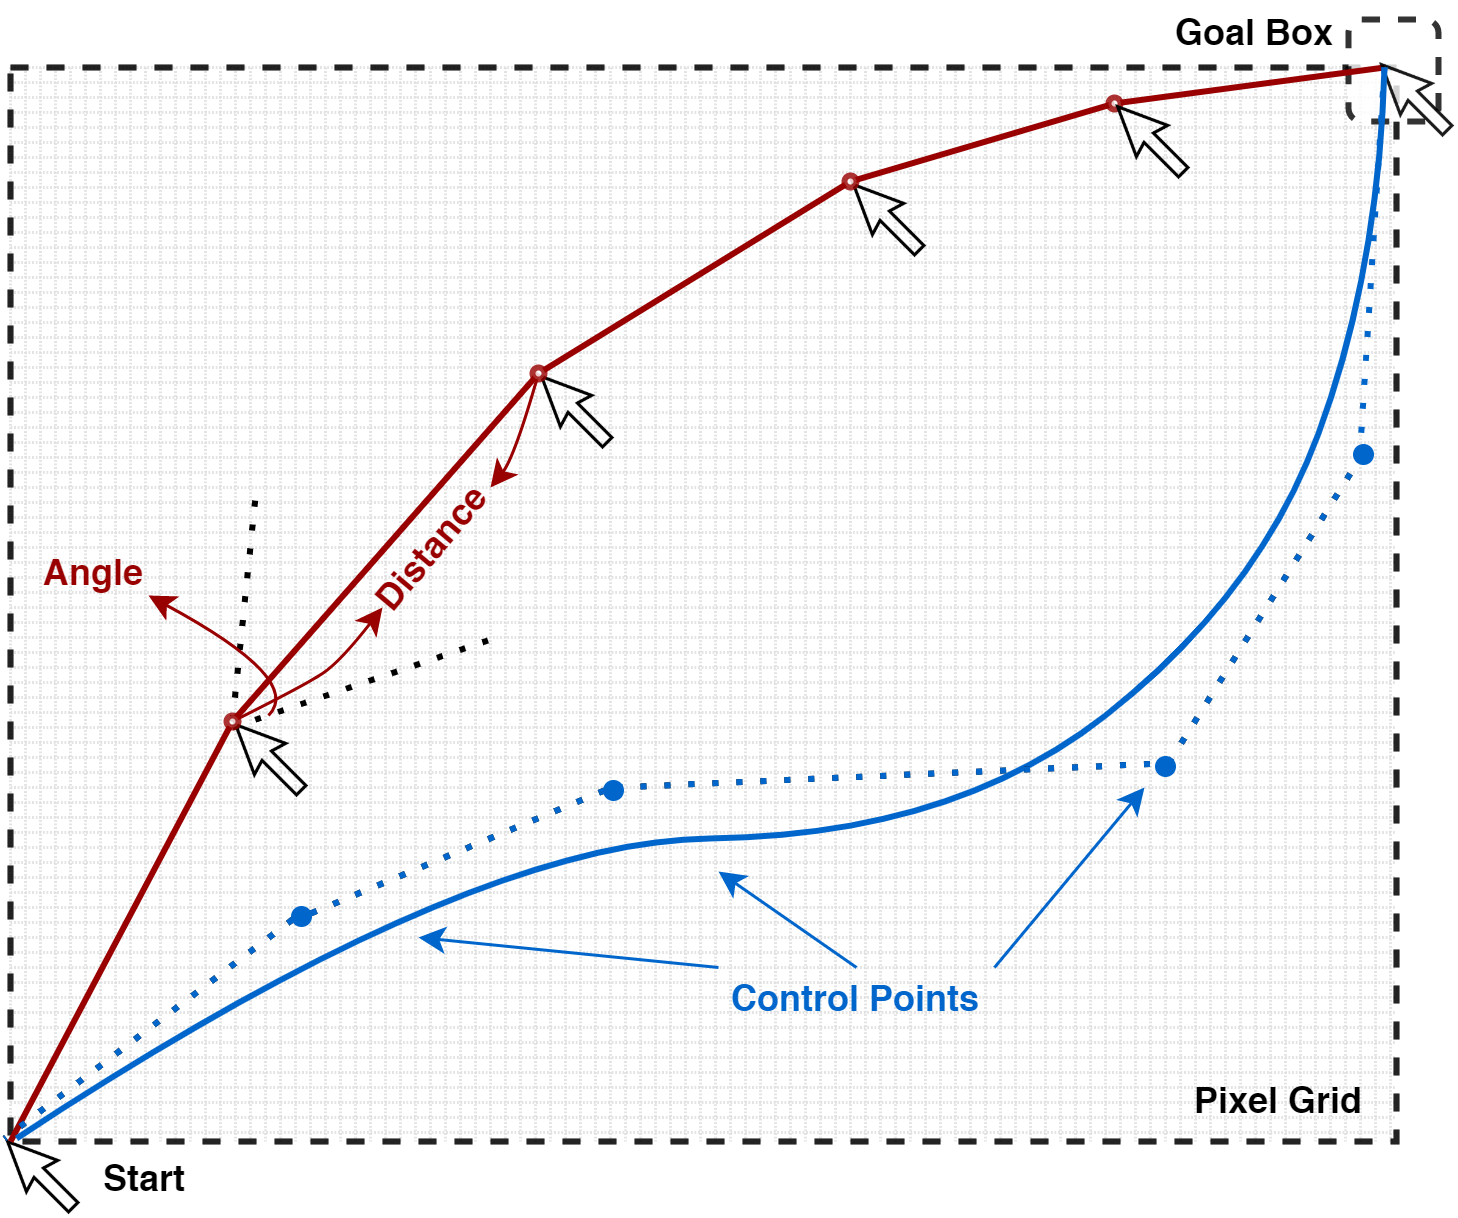
\includegraphics[width=0.95\columnwidth]{mouse.png}}
\caption{Agent controlled mouse movement. In red and blue are Piecewise and Bézier trajectories respectively.}
\label{mouse}
\end{figure}

\emph{Bézier.} We define a mouse trajectory from points $A \rightarrow B$ to be along the Bézier curve connecting $A$ and $B$ that is generated by control points chosen at random in the range $[A_x,B_x], [A_y,B_y]$.
We selected Bézier curves as they generate easy to parameterize smooth trajectories and are widely used in computer graphics and robotics \cite{tharwat2019intelligent, wang2020using}; a good fit for human-like mouse control, if not too good.
The agent controls 4 continuous values that are rescaled to the appropriate range.
Duration $d \in [0.5,1.5]$ that defines the trajectory speed, hover $h \in [0.2,1.1]$ that is the amount of time after the trajectory ends and before the mouse is clicked, press $p \in [0.05,0.55]$ that is the duration that the mouse button is pressed down, and delay $t \in [2,10]$ which is the amount of delay between each step/request -- listed timings are in seconds.
A sample trajectory is shown in Figure \ref{mouse}.

\emph{Abstract.} As in Bézier mode, in Abstract mode the agent controls 4 actions, with one key difference.
In place of delay $t$, at each step the agent now selects between 3 actions to perform; that is scrolling, typing, or mouse control which is carried out exactly like in Bézier mode.
All are parameterised by the duration, hover, and press values as before.
The value ranges of these actions are determined by studies carried out in related literature~\cite{dhakal2018observations, katerina2018mouse}.
For more information on these actions we refer the reader to Appendix \ref{appendix:b}.

\textbf{Reward}. The reward function embodies what we want the agent to learn or accomplish.
In our case the score is affected by a multitude of factors, and it can be a noisy signal to learn on, thus a simple reward mechanism would be most practical.
For Bézier and Abstract modes, the reward is the difference between the last received score and the average cumulative score the agent has received in this episode:

\begin{equation}
\begin{aligned}
    r_{BA} &= s_t-\overline{(s_{t-1}+\dots+s_0)}\\
\end{aligned}
\label{eqn:reward}
\end{equation}

where $s_t$ is the score at step $t$

In Piecewise mode, the reward is provided at the end of a trajectory/episode and is a weighted average of 3 terms: the difference between the current and last score, the amount of steps taken in order to incentivize precise trajectories, and a small constant term if the score remains high:

\begin{equation}
\begin{aligned}
    r_P &= s_t-s_{t-1} - 0.001\cdot N_t + 0.01\cdot h_t\\
    h_t &=
    \begin{cases}
      1, & \text{if}\ \geq 0.7\\
      0, & \text{otherwise}
    \end{cases}
    %r_1 &= w_1(s_t-s_{t-1})\\
    %r_2 &= -w_2 \cdot N_t\\
    %r_3 &= w_3 \cdot s_t, \forall s_t \geq 0.7\\
\end{aligned}
\label{eqn:rewre}
\end{equation}

where $s_t$ is the score at episode $t$ and $N_t$ is the number of steps in episode $t$.

\subsection{Algorithm}

To select an appropriate \gls{RL} algorithm for the environment, we need to take the properties of the environment into consideration.
As both state and action spaces are continuous, a value-based approach would be computationally intractable thus we opt for policy-based approaches \cite{sutton1999policy}.
Policy gradient methods optimize the policy $\pi_\theta(a|s)$ directly, where $\theta$ is usually approximated with neural networks, and they have been fundamental in recent breakthroughs in dynamical system control, 3D locomotion, and game playing.
Put simply, the neural network learns the optimal policy directly, i.e. which action $a$ to select in state $s$.
From the range of policy-based approaches, we conducted our experiments with the \gls{PPO} algorithm, specifically the PPO-Clip variant.
\gls{PPO} \cite{schulman2017proximal} is a state-of-the-art approach in \gls{RL} that solves many of the issues previous algorithms had, as it is simple to implement and tune, more general in the discovered policies, and has better sample complexity.
\gls{PPO} trains in an on-policy manner by sampling actions according to the latest version of its stochastic policy.
This policy is updated by maximizing the PPO-Clip objective function.
The reader is referred to Appendix \ref{appendix:a} for further information on the architecture and hyperparameters of our PPO agent.

The learning process for the Abstract agent is shown in Algorithm \ref{alg:abstract}, where: $n$ is the number of actions taken between each score request, $u$ is the number of steps between updates to the neural network parameterizing the policy, $M$ is the total number of episodes, $T$ is the maximum number of steps in an episode, and $a$ is the selected action.
The pseudocode for Piecewise and Bézier agents is included in Appendix \ref{appendix:a}.

To navigate web pages and the system interface in general, all agents receive $x,y$ values corresponding to absolute screen coordinates.
If the location within the screen is known in advance, coordinates are hard coded, otherwise they can be resolved through our browser extension that retrieves the location of HTML elements.

\begin{algorithm}
\SetAlgoLined
 Set number of steps $n$ per request\;
 Set policy update frequency $u$ in steps\;
 \For{episode $e$ = 1, 2, ... $M$ do}{
   Get initial score $S_0$\;
  \For{step $t$ = 0, 1, ... $T$}{
   Select action $a$\;
   Select duration $d$, hover $h$, press $p$\;
   Perform action $a$ parameterised by $d, h, p$\;
   \If {$t\pmod{u}== 0$}{
    Update policy and value networks based on Eq. \ref{appendix:objective} and Eq. \ref{appendix:value}\;
   }
   \If {$t\mod n == 0$}{
    Get score $S_t$\;
    Set $r_t$ based on Eq. \ref{eqn:reward}\;
   }
  }
 }
 \caption{PPO-Clip Abstract}
 \label{alg:abstract}
\end{algorithm}

\section{Evaluation}
\label{sec:evaluationrere}

In this section we elaborate on the empirical evaluations we performed and report on the results.
For the automated part of the experimentation, we use Firefox, Chrome, and Chromium as browsers, and a VPN service to shuffle our IP between browsing sessions.
We attempt to control for the score bias introduced by privacy settings by defining two distinct settings between browsing sessions, that is with third-party cookies disabled and private/incognito browsing enabled -- and vice versa.
The intent is to represent the differing levels of privacy-aware browsing behavior and serve as one form of introduced variance in order to observe the effect on the score.
Within each session, these configurations are kept constant as they represent the static, invariant aspect of browsing; our aim is to analyze how the risk analysis system is affected by controlling the interactive counterpart.
To avoid any validity threats in our methodology, browsers did not retain any state or information between sessions: if private/incognito mode was not enabled, cache and cookies were cleared after each.

\subsection{Empirical Evaluation}
\label{sub:empirical}

Throughout our experiments we spawn differently configured browsers on the same machine, so we investigated for potential tracking or cross-browser fingerprinting \cite{boda2011user}.
According to Google and Google Analytics documentation, Google can track unique IDs through their NID and SID cookies, with the stated intentions to authenticate users, prevent fraudulent use, perform targeted advertising, and others.
For the average web user, an effective, practical albeit counter-intuitive method against web tracking is by releasing more private information rather than less, as privacy-aware policies can make a user stand out in the crowd.
Previous work~\cite{sivakorn2016robot} studied the browser checks reCAPTCHA v2 performs, among them canvas fingerprinting \cite{mowery2012pixel}.
These checks are used to determine the existence of web automation frameworks or the browser version, and discrepancies can be highlighted by comparing the results to the reported user-agent.
During our empirical and automated evaluation, we did not observe signs either of tracking or of a detrimental effect to the score when the reported user-agent string was manipulated.

Before performing the automated evaluation, the first step is to observe how the risk analysis system is affected by the various browser configurations, the presence of cookies, different IP addresses, and more importantly user behavior during browsing.
We separate this information supplied to this system to its \emph{static} and \emph{dynamic} components.
Keeping all but one of the features constant while varying others provides us with practical insights as to how each one of them affects the score that each request gets.
More concretely we observe that:

\begin{itemize}
  \item Google cookies (GRECAPTCHA, NID \& SID) and enabled cookies in general have a decisive impact in the confidence of the system that the user is indeed human. This is to be expected, as cookies can track longer legitimate user activity.
  The experimentation with static features indicate that they affect the overall confidence of the system: when the confidence is high, dynamic features have little observable effect; conversely, when the confidence is low they appear to influence the score.
  The latter is also the setting we intend to induce and exploit in order to learn evasive human-like browsing behavior.
  \item Starting from a low score, something that occurs far more frequently with disabled cookies, we can consistently increase the score by engaging in typical browsing activity within the webpage, i.e. clicking, scrolling, typing in input fields, visiting subpages, etc.
  \item Starting from a high score, it is possible to diminish it either by overloading the webpage with requests or by performing bot-like actions with mouse and keyboard automation.
\end{itemize}

The scores returned by reCAPTCHA v3 are coarse-grained and do not fall in a continuous range: there are 4 discrete scores that a request can get: $S \in \{0.1, 0.3, 0.7, 0.9\}$.
A coarse-grained score offers two advantages in a Captcha system: (i) it simplifies for web administrators the process of drawing a threshold, and (ii) less information is divulged w.r.t. the model's decisions -- akin to gradient masking in adversarial \gls{ML}.

While high and low confidence refer to internal states of the risk analysis system that cannot be observed directly, a partial observation of them can be attained via the score behavior; high volatility in scores within a session indicates low confidence, while low volatility implies a high confidence state.
Through our empirical observations, we further delineate two more states, that can to a degree overlap with the high confidence state:
\begin{enumerate}
\item \emph{Score saturation}. Saturation occurs whenever the risk analysis system has a high level of confidence that the user is human.
This confidence may propagate to unrelated to the current session requests that come from different users.
In saturation, the score is insensitive to user dynamic behavior.
\item \emph{Score depletion}.
Depletion represents a high confidence that the user is a bot where all session requests receive the minimum score.
It can be caused by excessive requests -- hence the reason why frequency of requests is part of the variables controlled -- and it may propagate to unrelated requests irrespective of their source.
\end{enumerate}

This score behavior is extensively observed in both manual and automated experiments.
Naturally, from an adversarial perspective that intends to learn automated solutions a low confidence state is desirable and conducive to learning as it renders the score sensitive to user behavior.
It then follows that high confidence states can be also utilized as a deterrence against adversaries; for reCAPTCHA v2 this is explicitly disclosed by Google.
There is a prominent call in the Vulnerability Reward Program\footnote{https://bughunters.google.com/learn/invalid-reports/google-products/4539275112349696} to not submit reports when reCAPTCHA accepts invalid responses to challenges.
This explains that in order to combat automated solutions, if the system determines you are likely a human -- meaning it is in a state of high confidence/saturation -- it accepts even invalid answers.
Conversely, if it has high confidence that you are a bot, it rejects even correct answers.
The stated reasoning is that by always accepting correct and always rejecting incorrect answers, the challenge for adversaries is greatly simplified.

\subsection{Automated Evaluation}
\label{sec:auto}

\begin{figure*}[ht!]
\centerline{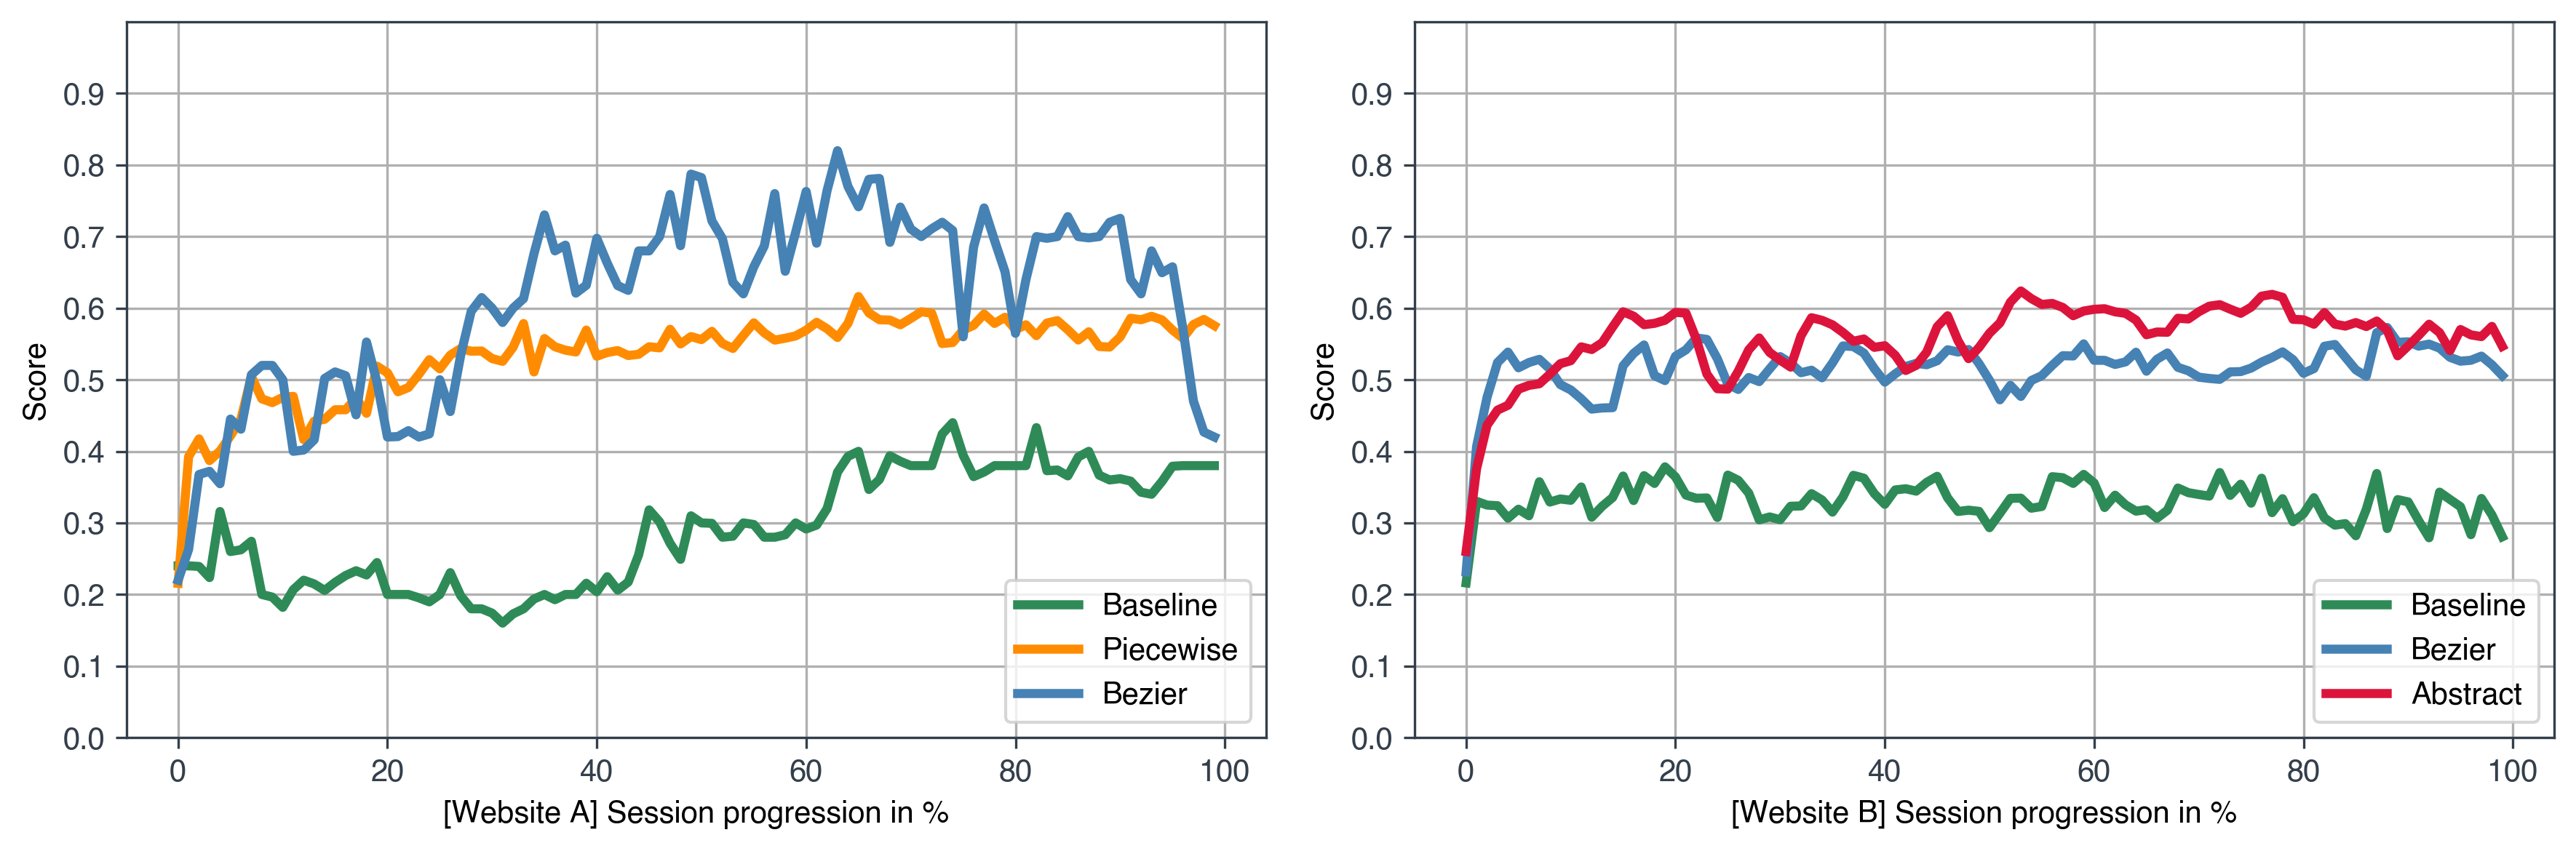
\includegraphics[width=0.95\textwidth]{SPPS.png}}
\caption{Score evolution in sessions initially flagged as bot, on Website A and Website B.}
\label{spps}
\end{figure*}

In all our experiments the automation is performed in a fully graphically enabled manner -- no headless browsers are used -- and the simulation of user browsing behavior is performed by programmatically controlling the mouse and keyboard.
The experiments spanned a period of 15 months, where more than 70K requests were submitted in total.
During this period, we progressively refine our agents with more general capabilities in order to encapsulate abstract, human-like browsing behavior.
To properly assess transferability and given the progressively more general agent capabilities, we conduct our evaluation in a cascading manner on three distinct web environments, as introduced in Section \ref{sec:approachre}:

\begin{itemize}
    \item Our self-hosted \textbf{Website A} which faces little actual traffic other than that from a few researchers, but where we had unconstrained request budget.
    Here Piecewise was in training \textit{and} testing mode, while Bézier solely in training.
    \item External \textbf{Website B} which sees considerable web traffic.
    On this website, the Bézier agent trained on Website A is now tested to evaluate how well it transfers, while Abstract is in training mode.
    \item External \textbf{Website C} which sees extensive web traffic.
    This website already had reCAPTCHA v3 integrated for bot protection, and the intention here is to evaluate how evasive is the Abstract agent trained on Website B.
\end{itemize}

The practical difference between training and testing mode is if the parameters of the policy network are updated or not, i.e. if any actual learning takes place.
Next to the RL-enabled agents, we implemented and evaluated on every website a \textit{Baseline} agent that differs in two key aspects: the mouse displacement is executed in a naive manner, i.e. either instantaneously or on a straight line connecting the origin and destination; additionally, no parameters are updated nor any learning of parameters happens.

\textbf{Website A}. On this website, next to v3 we additionally deploy reCAPTCHA v2.
The intention is to contrast their behavior throughout the evaluation.
As the authors in \cite{sivakorn2016robot} have demonstrated, when v2 has high confidence that the request is submitted by a human, it resolves to the ``no Captcha reCAPTCHA'' challenge that lets the user proceed without presenting a challenge.
reCAPTCHA v2 never resolved to ``no Captcha'' mode while v3 was in depletion, but surprisingly many times it did not resolve to ``no Captcha'' mode even when v3 was in saturation.
This indicates that the risk analysis systems behind the two versions of reCAPTCHA are potentially dissimilar in the way they process the information they collect as well as the risk profiles they build.

The main objective in this website is to have an initial estimation on how plausible the automated evasion of reCAPTCHA v3 is, but also whether we can learn from the score that the risk analysis system generates.
To investigate the hypothesis that the scoring system can be exploited, we utilize a \gls{VPN} service to intentionally search for and initiate sessions that start from a low score $s < 0.5$; more than two thirds of those sessions occur with disabled cookies and private/incognito mode.
Statistically throughout our experiments, low-starting sessions exhibit higher score volatility (about twice as much) indicating low-confidence states more sensitive to interactions.

In Figure \ref{spps} we illustrate the score evolution averaged over all such sessions, for each methodology we employed.
As sessions can have variable length, we normalize the time axis to a fixed $0-100\%$ range, and we calculate the average over this range.
There is a clear divide in performance between Baseline and both Piecewise and Bézier agents.
For the latter two, the score has a clear upwards tendency that on average surpasses the typical detection threshold within 20-25\% of a session's duration.
We observe a clear drop towards the end in the Bézier progression due to some sessions reaching more than 200 requests where the otherwise consistently high scores suddenly deplete to 0.1.
This is strong evidence that the temporal dynamics of incoming requests are taken into consideration, especially since it occurs at the \emph{same} time irrespective of which session we submit the requests from.
Figure \ref{swos} plots the average cumulative score each methodology achieves over the period of evaluation.
Once again there is a clear divide between the Baseline and the \gls{RL} enabled agents, with Bézier being the approach getting most consistently high scores.

\begin{figure*}[ht!]
\centerline{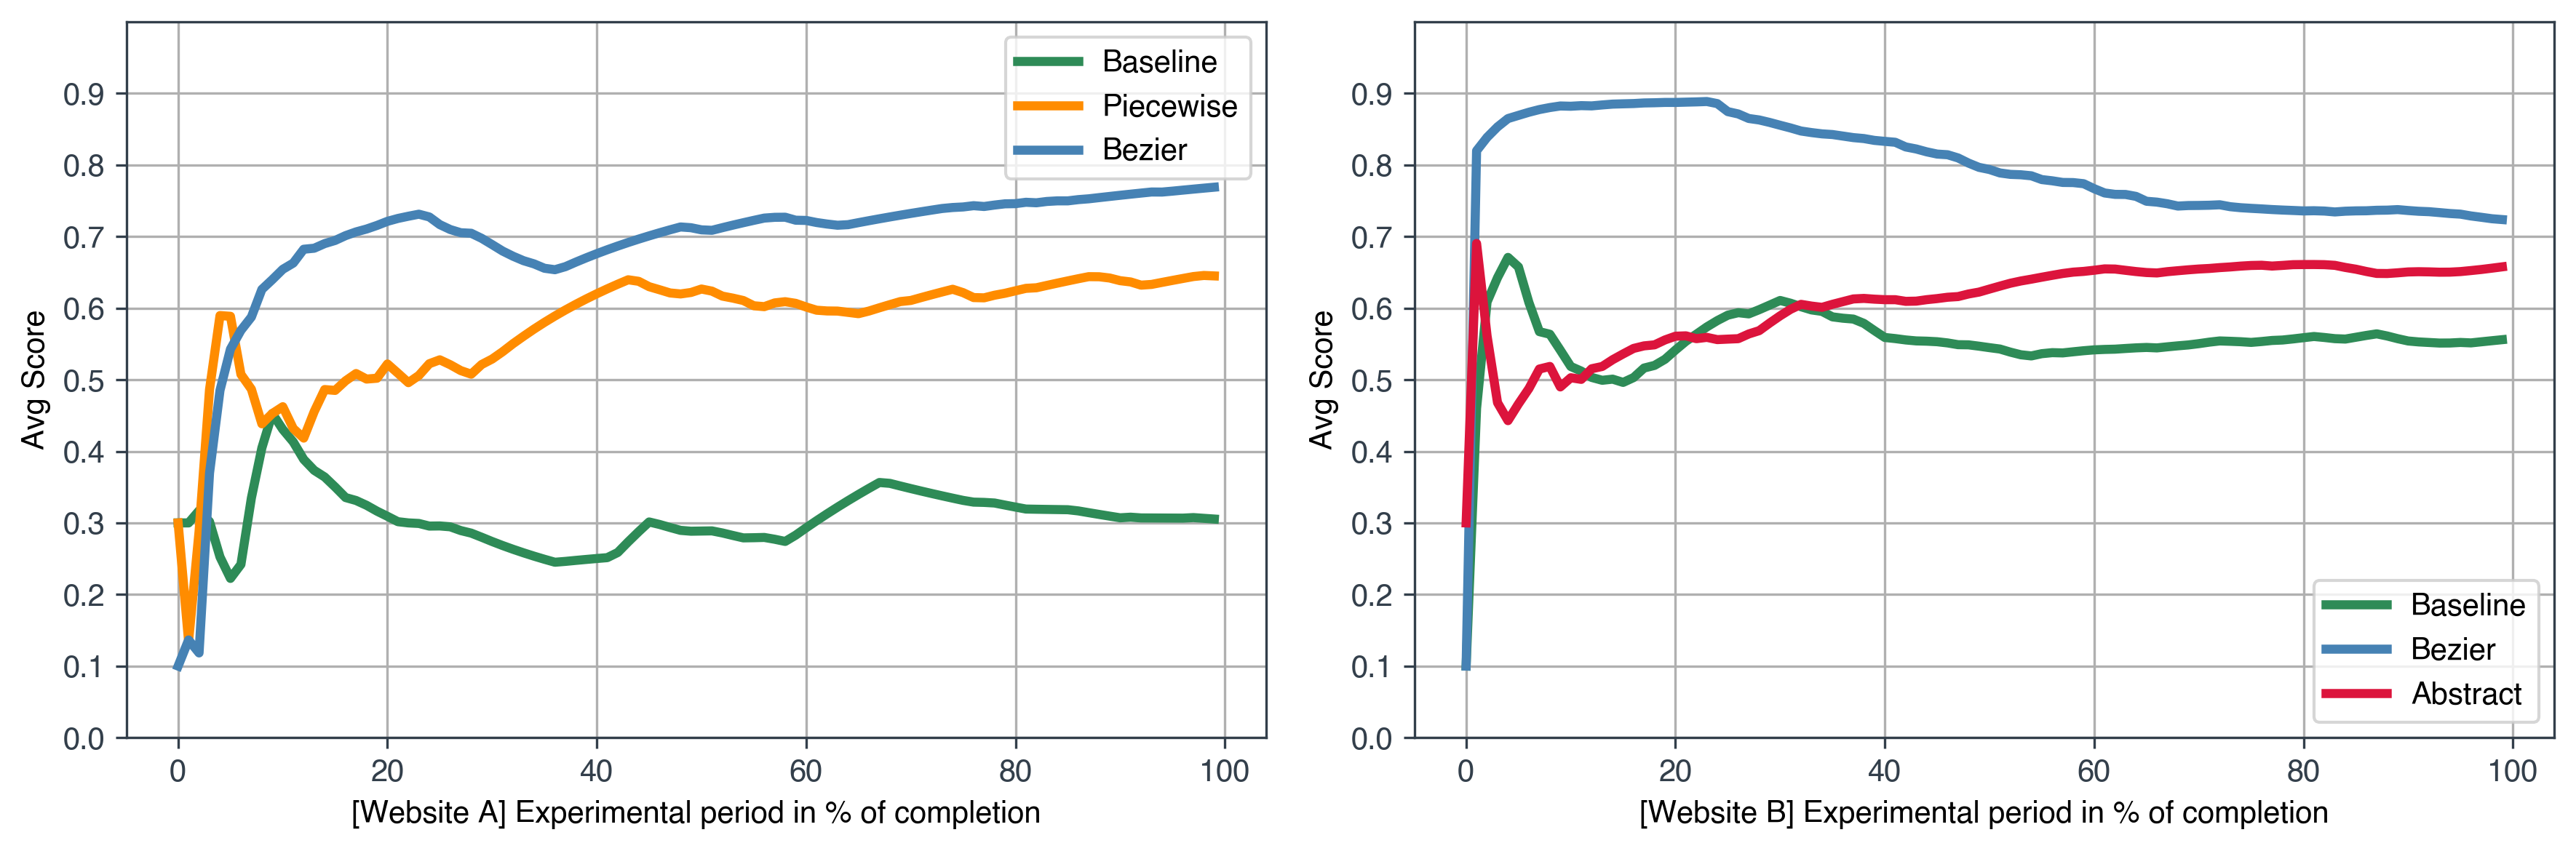
\includegraphics[width=0.95\textwidth]{SWOS.png}}
\caption{Average cumulative score over the period of evaluation, for Website A and Website B.}
\label{swos}
\end{figure*}

\textbf{Website B}. As website A is practically a synthetic one, albeit one that offers ease of access and unconstrained querying, it is probably not representative of the whole as the risk analysis system adapts by observing actual traffic.
To properly evaluate the capabilities of our automation and put this to the test, we transition our experimentation to Website B as it faces actual live web traffic.
As described in Section \ref{sec:approachre}, in coordination with the administrators we deploy reCAPTCHA v3 on the website and wait for 1 week until it models the traffic patterns to avoid skewing them.
In this setting, we evaluate how well the most performing agent trained on Website A transfers to the new context; that is without using the scores and without further re-training or fine-tuning.
Additionally, we ascertain if an even more general and evasive model can be learned.

In Figure \ref{spps} we illustrate the score evolution averaged over all sessions that start below the bot threshold -- 96 out of 180 -- for each methodology we employed.
We observe a clear but less prominent gap between the Baseline and the \gls{RL} enabled agents.
In this environment saturation and depletion still occur but differently than on Website A.
While it is still possible to deplete the score due to an overabundance of requests, when it happens it concerns only the IP address where the requests were submitted from and does not propagate to others.
The sessions where the score reached depletion due to excessive requests were less than 3\% of the total.

In Figure \ref{swos} we illustrate the average cumulative score each methodology achieves over the period of evaluation.
One thing we immediately observe is that Bézier performs the best out of the box, however Abstract diminishes the gap over time as the Bézier agent no longer updates its parameters.
Another notable observation in this web environment is that the baseline is comparable to the \gls{RL} methodologies.
This indicates that even a rudimentary GUI-enabled automation can be sufficient to consistently evade reCAPTCHA v3 detection.

\textbf{Website C}. After concluding our experiments on Website B, we want to assess the level of threat our \gls{RL} enabled automation poses on the web.
The best candidate is the Abstract agent: it incorporates common browsing capabilities that so far were scripted when needed, and is thus the most general model we created.
The next step is to evaluate its evasive performance and the degree this transfers to websites that get considerable traffic.
Furthermore, our intention is to obviate any kind of learning and to transition to the fully black-box case.
Website C is an ideal candidate as compared to B gets two orders of magnitude more daily requests.
In contrast to Website B, scores are no longer accessible.
There is only a visible indicator that shows whether the score was above an unspecified threshold or not: the intention is to reflect attack scenarios on other websites where we have no access to the scores, only the binary verdict if further verification is required.
Unlike previous websites where we track the average score, on Website C we report the percentage of requests that go undetected instead, denoted as evasion rate.

We evaluate the Baseline and Abstract agents in two principal contexts that aim to reflect and contrast the worst and best cases for the adversary: sessions that are initially flagged as bot (low starting) and not (high starting) respectively.
Compared to A and B, it is exceedingly more difficult to find low starting sessions on Website C.
The results are included in Table \ref{tab:requests}.
We notice that for low starting sessions, the performance gap between Baseline and Abstract is quite prominent, while for high starting sessions less so.
For high starting sessions, that adversaries have ample opportunity to initiate, the Abstract agent goes almost completely undetected with an evasion rate of 99.6\%, while even the Baseline agent reaches an evasion rate of 84.3\%.
This demonstrates a stark decline on the level of bot mitigation that reCAPTCHA v3 offers, and a clear vulnerability that an attacker with sufficient resources can exploit.

\subsection{Explainability}

Despite the overall success that our approach has in evading detection and in exposing a vulnerability at the core of how such a bot detection scheme functions, some open questions remain:
\begin{itemize}
    \item What is the risk analysis system behind reCAPTCHA v3 scoring exactly?
    \item Apart from demonstrating the vulnerability itself, can we obtain a deeper understanding of what is happening within the black box?
    \item Which aspects of our online behavior influence the score, and to what degree each?
\end{itemize}

During the evaluation on Website B, we registered about 13K requests in total.
From these requests, we generated a dataset where each instance contains the following information:
\begin{enumerate*}
    \item The duration for which actions execute.
    \item The hover timing.
    \item The press timing.
    \item The delay between successive requests.
    \item The presence of cookies.
    \item The frequency of requests.
    \item The time in the day.
    \item The day of the week.
    \item The number of different actions used.
    \item The total number of requests submitted in current session.
    \item The score that the request got.
\end{enumerate*}

In order to get insights into how does reCAPTCHA v3 score requests, an intermediary step is to extract a functionally equivalent model that shadows the decisions of reCAPTCHA v3 \cite{jagielski2020high, bastani2017interpreting}.
The abundant data we collected during our experiments provided such an opportunity.
We train Random Forest (\gls{RF}) classifiers and regressors~\cite{liaw2002classification} with the aforementioned features as independent variables and the score as the target variable.
On the classification task we reach $87.5\%$ mean accuracy and on the regression task we reach $0.82$ $R^2$.
In practical terms, an $R^2$ of $0.82$ indicates that the model cannot explain $18\%$ of the variability in the outcome.
This is anticipated as Google has access to a broader set of information that in our models cannot be accounted for.
Examples are the reputation of IP addresses and ranges, deviation from heatmaps generated through Google Analytics for that particular website, and spatial, temporal or entropic aspects of user activity.
The above are either missing or confounding variables, so we note to the reader here that a statistical analysis can indicate but does not entail causal properties~\cite{scholkopf2019causality}.

\begin{figure}[b]
\centerline{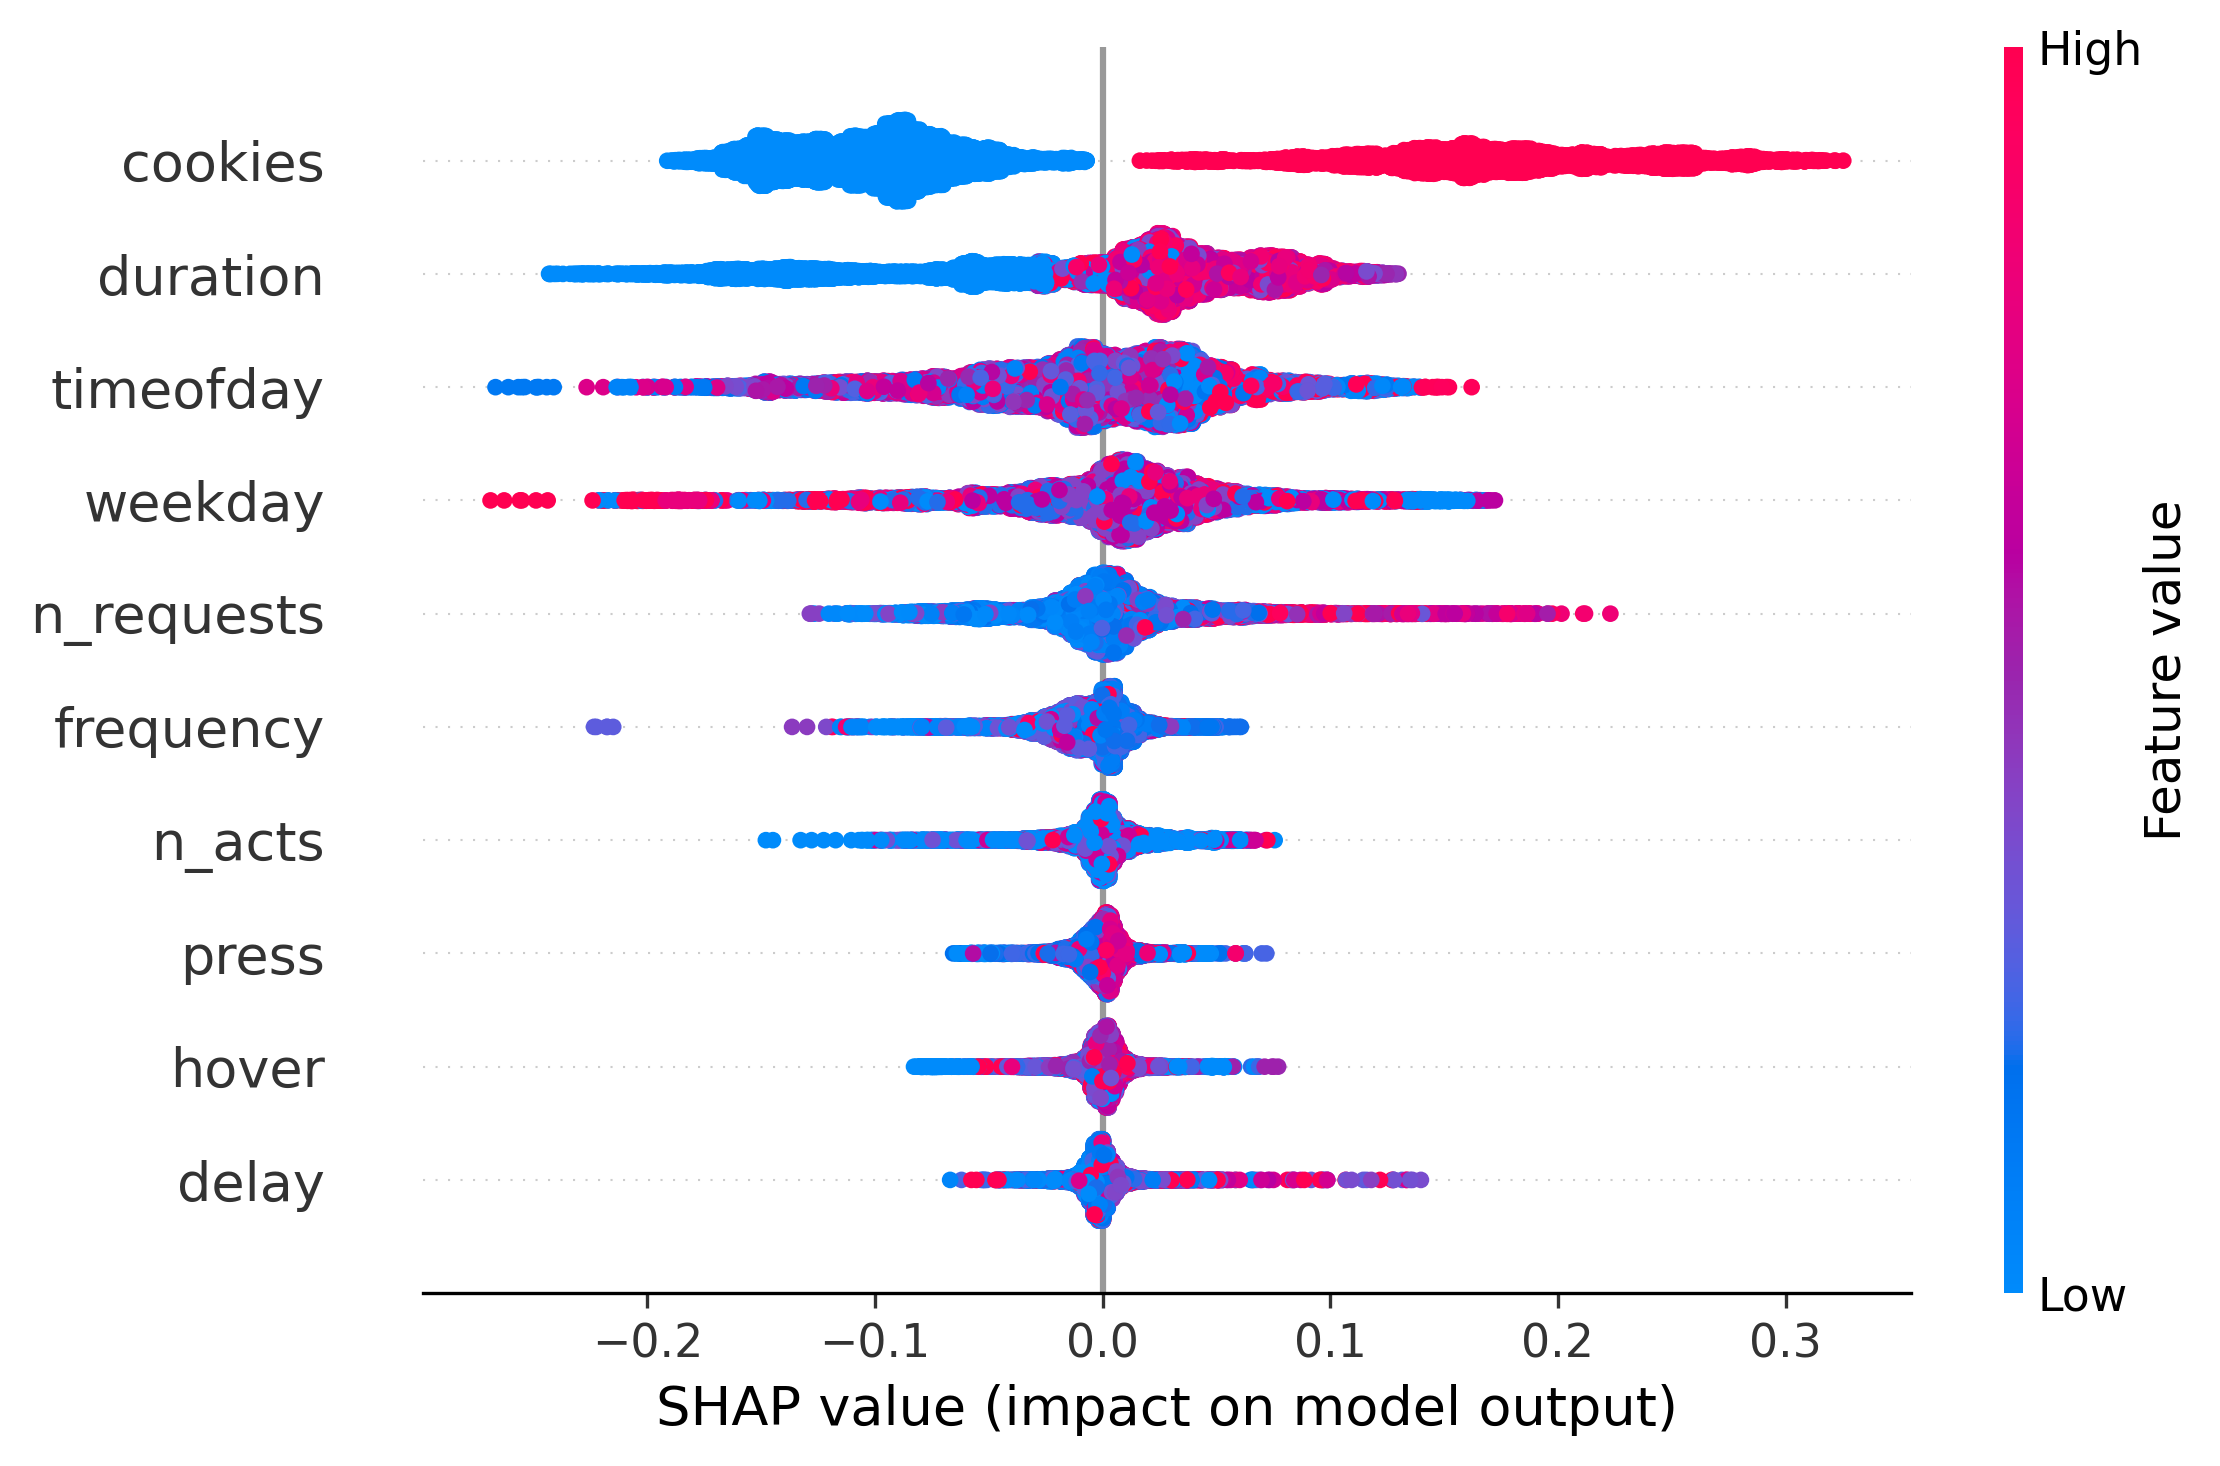
\includegraphics[width=0.95\columnwidth]{SHAP.png}}
\caption{Shapley values for all features, depicted in descending order of importance}
\label{shap}
\end{figure}

Our goal however is not to extract a high-fidelity model of the risk analysis system behind reCAPTCHA v3, but to get a glimpse in the black box and explain how various factors can influence the score; factors that come as a result of our initial assumptions.
To that end we employ a powerful framework for explainable AI called SHapley Additive exPlanations (SHAP), a game theoretic approach to explain the output of any \gls{ML} model.
SHAP connects optimal credit allocation with local explanations using the Shapley values, i.e. the average of the marginal contributions of the features, across all the feature permutations \cite{lundberg2017unified}.
We note here that by following an experimental protocol, bias is inadvertently introduced in the collected data.
For instance, the effect of the presence of cookies will be exaggerated; we searched for low starting sessions, something that occurs considerably more often with disabled cookies.

Figure \ref{shap} demonstrates how each variable influences the score, in descending order from most to least influential.
The presence of cookies is the most influential, indicating that the risk analysis system has a clear bias between more and less privacy-aware web browsing behavior.
What is interesting though is duration at the second spot and that it is positively correlated with the score.
This indicates that short or instant actions are biasing the score to lower values.
Time of day and weekday are also influential; their influence is most probably overestimated as we unintentionally introduce some bias by following typical (mostly) office activity.
The number of requests is counter-intuitive at first; while a few high values are correlated with low scores, indicating depletion, the feature is mostly positively correlated with score, indicating that longer and human-like activity is a strong predictor of higher scores.
The number of actions has a slight and positively correlated influence, corroborating our findings that put the Abstract mode a step above Bézier.
What is unexpected here though is that mouse button press, mouse hover, and the delay between requests have little to no influence to the model.
The value ranges of press and hover are, by our definition, commensurate to the average human ones; they might as well be completely decoupled from the score. 

\textbf{Computational cost}. Throughout our experiments, the most demanding agent computationally was Piecewise, as it had to control actions at a rate of 50 FPS required for seamless trajectories.
The computational bottleneck here is the neural network behind the agent policy, and the average inference time on an Intel i7-7700 CPU was $5 \times 10^{-4}$ seconds which could theoretically support up to 2000 FPS control.
Regarding the implementation and evaluation platforms, all scripts and \gls{RL} agents were written in Python while a browser extension written in JavaScript was used to retrieve scores -- all experiments were carried out on a dedicated desktop machine with Ubuntu 18.04.

In Table \ref{tab:requests} we report the summary on the scores, numbers of requests, and overall traffic, across all experiments and for each of the websites.
Over a period of 15 months, our \gls{RL} enabled methodology successfully used the risk analysis system behind reCAPTCHA v3 to learn evasive models of web browsing, while submitting high numbers of requests commensurate to the total traffic a website attracts.

\begin{table*}
\centering
   \begin{tabular}{lccc|ccc|cc}
    \toprule
    &
      \multicolumn{3}{c}{Website A} &
      \multicolumn{3}{c}{Website B} &
      \multicolumn{2}{c}{Website C}\\
      & \small {Base} & \small {Piece} & \small {Bézier} & \small {Base} & \small {Bézier} & \small {Abstract} & \small {Base} & \small {Abstract}\\
      \toprule
    $S_L$ & 0.22 & 0.52 & 0.60 & 0.33 & 0.60 & 0.58 & 20.8\% & 70.1\%\\
    $S_T$ & 0.31 & 0.65 & 0.77 & 0.56 & 0.72 & 0.66 & 51.6\% & 90.0\% \\
    $S_H$ & 0.52 & 0.71 & 0.83 & 0.73 & 0.86 & 0.80 & 84.3\% & 99.6\% \\
    \midrule
    $R_T$ & 2.6K & 21K & 8K & 6.3K & 4.4K & 2K & 8.6K & 12.4K\\
    $R_D$ & 130 & 231 & 244 & 203 & 182 & 89 & 866 & 773 \\
    $R_S$ & 101 & 140 & 144 & 93 & 75 & 37 & 208 & 122\\
    $D_S$ & 203 & 761 & 526 & 40 & 71 & 37 & 68 & 136\\
    % $N_D$ & & 92 & 33 & 31 & 24 & 22 & & & & 8\\
    \midrule
    $T_T$ & -- & -- & -- & 12.3K & 9.4K & 9.3K & 328K & 413K \\
    $T_D$ & -- & -- & -- & 398 & 390 & 421 & 33K & 26K\\
    \bottomrule
  \end{tabular}
  \caption{Requests per website and agent. $S_L$, $S_T$, $S_H$ are the average score for low starting, total, and high starting sessions respectively. For Website C, $S_L$, $S_T$, $S_H$ denote the evasion rate instead. $R_T$ is the total amount of requests, $R_D$ are the average requests per day, $R_S$ are the average requests per session, $D_S$ is the average session duration in minutes, $T_T$ and $T_D$ are the total and daily amount of traffic during the experiments.}
  \label{tab:requests}
\end{table*}

\section{Discussion}
\label{sec:discussionre}

In this section we critically reflect on the results and provide further insights into the topic.
Captcha solutions are an essential tool to combat bot proliferation on the internet and the financial or other harm they may cause.
From fraudulent transactions, to credential stuffing attacks and click fraud, an adversary would benefit immensely from general and human-like web browsing policies that evade Captcha detection.
The ability to learn such a behavior by utilizing a popular, widely used Captcha service as an oracle, is a clear vulnerability that needs to be addressed as it can constitute the main component of a system that automates web attacks.
Transitioning from one-shot Captcha challenges to overall behavior monitoring has another implication.
If human behavior and its imitation are indistinguishable to such a detection scheme, then this scheme -- aside from being insufficient -- enables the perfection of this imitation.

In January 2020 Google launched reCAPTCHA Enterprise, where this vulnerability could potentially be more severe.
According to the documentation, reCAPTCHA Enterprise appears to be based on reCAPTCHA v3, with some modifications that intend it towards enterprises.
Like v3, reCAPTCHA Enterprise will never interrupt users with a challenge, but it includes a pricing for every 1K requests submitted above 1M per month.
Additionally, potential customers have to supply personal and company information for a vetting process.
A key difference to reCAPTCHA v3 is that now the scores returned include reason codes.
These codes provide information on the reason reCAPTCHA Enterprise interpreted the interaction that way, in practice embedding explainability into the inference process.
Such reason codes are:
\begin{itemize}
  \item \textit{automation}, when an automated agent is detected.
  \item \textit{unexpected\_environment}, when an illegitimate environment is detected.
  \item \textit{too\_much\_traffic}, when the traffic volume from a specific source exceeds typical values.
  \item \textit{unexpected\_usage\_patterns}, when interactions in the website diverge significantly from expected patterns.
  \item \textit{low\_confidence\_score}, when there is insufficient traffic observed to generate a representative risk score.
\end{itemize}
There are several surprising correspondences between these reason codes and our findings while investigating the risk analysis system of reCAPTCHA v3, for instance \textit{too\_much\_traffic}.
An adversary with access to such explanations behind the black-box decision acquires a more fine-grained reason to what effect their actions have and a learning signal to optimize the parameters of an offensive methodology even more effectively.
However, putting a premium on requests and putting customers through a vetting process can disincentivize that.
This indicates a promising path for future work.

\textbf{Ethics}.
Before deploying reCAPTCHA v3 on Websites B and C, we acquired explicit consent from the owners and administrators.
Regarding the potential impact on these websites, an open question was how will our automated activity affect the scores of unrelated requests and overall user experience, even considering that a low score will not mean escalation to further verification in neither website.
After all, depletion is a prominent phenomenon on Website A, so we wanted to be extra careful when we proceeded to actual websites with considerable live traffic.
In contact with the website administrators, we set an initial conservative threshold on the amount of queries submitted to be in par with the daily traffic, and gradually increased it.
In case of depletion we agreed to slow our requests down to a halt in order to investigate the cause and analyze the impact; something that ultimately did not occur.

\textbf{Responsible Disclosure}.
Regarding the broader impact that our evasion attack on Google reCAPTCHA v3 can have, we followed the standard responsible disclosure policy: we notified Google of our findings and the vulnerabilities we discovered in reCAPTCHA v3.
Google responded to our detailed report and acknowledged the vulnerability.
After further investigation on their side, Google has closed the issue without providing a fix and the status code ``intended\_behavior''.
We surmise that acquiring access to backend scores and that fully graphically enabled automation attacks are considered reasonable limitations on the adversary, however at the time of publication these issues were still present.

\textbf{Defenses}. As our methodology does not tinker with the HTTP requests or cookies, defenses would fall primarily within the adversarial training paradigm~\cite{tramer2017ensemble}, that is to train the model with data that were specifically created to fool it.
The explicit goal is to make the risk analysis system more robust towards adversarial activity.
This however is a complicated matter as the domain of Captcha is considerably broader than image classification.
No matter its abstraction or representation, the distribution of human behavior online is expected to be fairly diverse for adversarial examples -- adversarial behavior here -- to hide in the crowd.
As adversarial examples are fundamentally \gls{OOD} data~\cite{geirhos2020shortcut}, proactively modeling them can be a challenging task.
There is however precedence in utilizing adversarial examples as Captcha resilient to automated solutions~\cite{osadchy2017no}.
Finally, as long as one can obtain oracle access to the risk analysis system, defenses are limited to obfuscation and rate limiting.
Adversaries can iteratively refine their attacks by using the oracle as either a discriminator to a \gls{GAN} approach or a reward function to a policy gradient method.

\textbf{Limitations}. The most capable agent demonstrates that it is possible to fully evade detection on a website of which it had zero beforehand knowledge or interaction with.
However, in order to fully exploit the information leakage in reCAPTCHA v3, and in case the initial evasive policy is insufficient, an adversary would have to have access to the oracle for longer periods of time; something made evident by the evolution of scores in Figure \ref{swos}.
Furthermore, we posit that while the score returned by v3 is a signal that allows learning to take place, it is still one with noise, or as Google has indicated for v2, at times even intentionally misleading.
If other heavily influencing factors are not controlled for, this innately limits the degree that learning can take place.

In many configurations, e.g. with low privacy settings, the baseline approach was sufficient to evade detection, up until depletion.
Beside the effectiveness and transferability of our approach, our results underline the importance of developing the scientific understanding of the strengths and limitations in the new paradigm of frictionless Captcha, specifically in the presence of adaptive attackers capable of learning from interaction with the deployed detection mechanism.

\textbf{Controversies}. While widely useful and an important pillar in the fight against bots and malicious users, Captcha does not come without its controversial aspects.
reCAPTCHA was rightfully criticized for being a source of unpaid work to assist in transcribing text and image labeling tasks.
As a competing solution, hCaptcha\footnote{https://www.hcaptcha.com/} raison d'être is to change this by returning some of the revenue made from solving the Captcha to the website owner.
What can be disconcerting though is that frictionless Captcha such as reCAPTCHA v3 and Enterprise, amass a great wealth of information by monitoring all the interactions occurring in a website.
As automated solving becomes ever more efficient and effective, Captchas transitioning towards behaviometrics, where there is no longer revenue to be made by transcribing text or labeling images.
In this case, the users' online behavior could become the revenue, this time not to commercialize insights but as Turing tests.

\textbf{Availability \& Future Work}.
We opt for \gls{RL} as a learning paradigm as it enables optimal behavior without access to gradients; the agent can learn in an immediate, online manner by interacting with the environment.
Our approach and general framework are modular by design to accommodate the learning of any parameters that might affect the risk analysis scoring system, in the case it adapts to observing a broader or different set of information.
As a result, there are two primary promising paths for future exploration:
First, the possibility to train more capable agents by exploiting the reason codes of reCAPTCHA Enterprise.
Secondly, to explore more effective defenses that go beyond rate limiting and security by obscurity, in the domains of adversarial \gls{ML} and competitive multiagent \gls{RL}.

\section{Conclusion}
\label{sec:conclusion}
This work presents the first comprehensive investigation of Google reCAPTCHA v3 service.
Over various websites, web configurations, attack methodologies and a period of fifteen months, we perform a black-box analysis and comprehensive evaluation of the risk scores reCAPTCHA v3 generates.
We discover that it offers insufficient protection against web automation as we are able to consistently bypass it with an evasion rate up to 99.6\%.
We evaluate how different aspects of the activity on a website protected by reCAPTCHA v3 influence the score.
Static aspects like privacy settings and IP address have a constant positive or negative impact on the score and do not change during a session.
On the other hand, the score is also influenced by volatile aspects directly linked to the dynamic browsing behavior of the user.
As reCAPTCHA v3 constantly monitors user interactions to differentiate between humans and bots by generating a risk score, we exploit this information to learn a general model of automated web browsing that consistently evades detection.

Our study indicates that while a transition towards Captcha services based on continuous behaviometric evaluation is unavoidable, as text and image Captchas have become more difficult for humans to solve than for AI, this inadvertently leads to vulnerabilities that dedicated adversaries can potentially exploit.
The effectiveness of our approach demonstrates the need for improved bot and automation detection in zero friction, zero challenge Captcha.
Nevertheless, as this type of Captcha are becoming more prominent, the competition in differentiating between human interaction and its imitation accelerates and calls for further research on proactive and reactive response to such adversarial activity.